\documentclass[aspectratio=169,10pt]{beamer}
\usepackage[T1]{fontenc}
\usepackage{amsmath,amssymb,amsfonts}
\usepackage{bm}
\usepackage{tikz}
\usepackage{xcolor}
\usetikzlibrary{arrows.meta,positioning,shapes,calc}

\definecolor{parchment}{HTML}{F4E8C8}
\definecolor{paper}{HTML}{FAF1D8}
\definecolor{ink}{HTML}{1A1A1A}
\definecolor{inkgray}{HTML}{5A5A5A}
\definecolor{accentred}{HTML}{8B1A1A}
\definecolor{accentgreen}{HTML}{2D5F2C}
\definecolor{accentblue}{HTML}{1F4E79}
\definecolor{redbg}{HTML}{F7E0DE}
\definecolor{grnbg}{HTML}{E0EBDC}
\definecolor{blubg}{HTML}{DDE6EF}
\definecolor{labelbg}{HTML}{EFE0B0}

\usefonttheme{serif}
\setbeamercolor{background canvas}{bg=parchment}
\setbeamercolor{normal text}{fg=ink}
\setbeamercolor{structure}{fg=ink}
\setbeamercolor{frametitle}{fg=ink,bg=parchment}
\setbeamercolor{title}{fg=ink}
\setbeamercolor{itemize item}{fg=ink}
\setbeamercolor{itemize subitem}{fg=ink}
\setbeamercolor{item}{fg=ink}
\setbeamercolor{caption name}{fg=ink}
\setbeamertemplate{navigation symbols}{}
\setbeamertemplate{itemize item}{\textbullet}

\setbeamertemplate{frametitle}{%
  \vspace{0.30em}%
  \begin{center}%
    {\bfseries\Large\insertframetitle\par}%
    \vspace{0.28em}%
    {\color{ink}\rule{0.86\paperwidth}{0.4pt}}%
  \end{center}%
  \vspace{0.10em}%
}
\setbeamertemplate{footline}{%
  \hbox to \paperwidth{\hfil\itshape\small\insertframenumber\hspace{0.7em}}%
  \vspace{0.35em}%
}

\newcommand{\vY}{\bm{Y}}
\newcommand{\vy}{\bm{y}}
\newcommand{\vA}{\bm{A}}
\newcommand{\vB}{\bm{B}}
\newcommand{\valpha}{\bm{\alpha}}
\newcommand{\vn}{\bm{n}}
\newcommand{\vs}{\bm{s}}
\newcommand{\vW}{\bm{W}}
\newcommand{\T}{^{\mathsf T}}
\newcommand{\Hh}{^{\mathsf H}}
\newcommand{\norm}[1]{\left\lVert #1\right\rVert}
\DeclareMathOperator*{\argmin}{arg\,min}

\tikzset{
  flowbox/.style={draw=ink,fill=paper,line width=0.6pt,
                  minimum width=2.5cm,minimum height=1.0cm,
                  align=center,font=\small\bfseries,inner sep=4pt},
  smallbox/.style={draw=ink,fill=paper,line width=0.4pt,
                   minimum width=0.7cm,minimum height=0.55cm,
                   inner sep=2pt,align=center,font=\footnotesize\itshape},
  method/.style={draw=accentgreen,fill=grnbg,line width=1.0pt,
                 align=center,font=\small\bfseries,inner sep=6pt},
  issue/.style={draw=accentred,fill=redbg,line width=1.0pt,
                align=center,font=\small\bfseries,inner sep=6pt},
  idea/.style={draw=accentblue,fill=blubg,line width=1.0pt,
               align=center,font=\small\bfseries,inner sep=6pt},
  flowarr/.style={-{Stealth[length=2.5mm,width=2mm]},line width=0.7pt},
  softarr/.style={-{Stealth[length=2mm,width=1.6mm]},line width=0.5pt,color=inkgray}
}

\newcommand{\bottomnote}[1]{%
  \begin{center}{\itshape\small #1}\end{center}}

\newcommand{\papercover}[4]{%
  \begin{frame}[plain]
    \vfill
    \begin{center}
      {\bfseries\Huge #1\par}
      \vspace{0.8cm}
      {\Large #2\par}
      \vspace{0.35cm}
      {\itshape\large\color{inkgray}#3\par}
      \vspace{0.55cm}
      {\small\texttt{\detokenize{#4}}\par}
    \end{center}
    \vfill
  \end{frame}}

\newcommand{\twocolmodel}[4]{%
  \begin{columns}[T,onlytextwidth]
    \begin{column}{0.48\textwidth}#1\end{column}
    \begin{column}{0.48\textwidth}#2\end{column}
  \end{columns}
  \bottomnote{#3\\#4}}


\begin{document}

\papercover
  {Partial-Band Interference Cancellation}
  {Zhaohui Wang, Shengli Zhou, Catipovic, and Willett}
  {IEEE Transactions on Signal Processing, 2012}
  {partial_band_interference_ofdm_uwa.pdf}

\begin{frame}{1. Core Problem}
\twocolmodel{
  \begin{itemize}\setlength{\itemsep}{0.45em}
    \item UWA links can be hit by external signals such as sonar or jamming.
    \item The interference may occupy only part of the band and part of the OFDM block.
    \item Treating it as ordinary noise wastes structure.
  \end{itemize}
}{
  \[
    \vy=\vA\vs+\vB_{\rm int}\valpha+\vn
  \]
  \[
    \vB_{\rm int}
    =
    \text{known time-frequency support basis}
  \]
}{
  The interference is unknown, but its time-frequency footprint can be parameterized.
}{
  Estimate the communication signal and the external waveform together.
}
\end{frame}

\begin{frame}{2. Iterative Receiver}
\begin{center}
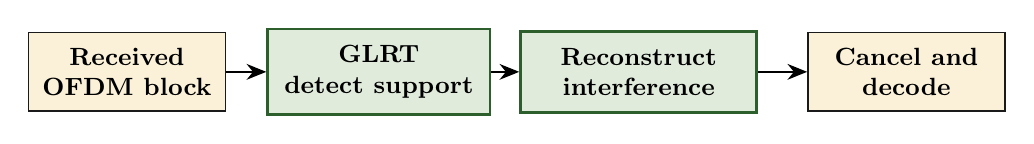
\begin{tikzpicture}[x=1cm,y=1cm]
  \node[flowbox] (rx) at (-5.2,0) {Received\\OFDM block};
  \node[method,minimum width=2.8cm] (glrt) at (-2.0,0) {GLRT\\detect support};
  \node[method,minimum width=3.0cm] (ls) at (1.3,0) {Reconstruct\\interference};
  \node[flowbox] (clean) at (4.7,0) {Cancel and\\decode};
  \draw[flowarr] (rx) -- (glrt);
  \draw[flowarr] (glrt) -- (ls);
  \draw[flowarr] (ls) -- (clean);
\end{tikzpicture}
\end{center}
\[
  \widehat{\valpha}
  =
  \argmin_{\valpha,\vs}
  \norm{\vy-\vA\vs-\vB_{\rm int}\valpha}_2^2
\]
\bottomnote{The GLRT supplies structure; least squares supplies waveform amplitudes; decoding supplies better symbol estimates for the next pass.}
\end{frame}

\begin{frame}{3. Why It Works}
\begin{itemize}\setlength{\itemsep}{0.48em}
  \item The interference is low-dimensional once its occupied band and time duration are known.
  \item Nulls, pilots, and tentative decisions expose interference energy.
  \item Reconstruction prevents the receiver from confusing external energy with channel taps.
  \item Iteration improves both communication decoding and interference cancellation.
\end{itemize}
\bottomnote{The paper separates ``channel physics'' from ``environmental intrusion'' by giving the intrusion its own model.}
\end{frame}

\begin{frame}{4. JUNA Connection}
\begin{itemize}\setlength{\itemsep}{0.5em}
  \item JUNA should include nuisance variables for structured interference:
  \[
    \vY_k=\sum_q\bm c_{kq}s_q+\bm b_k\alpha+\vn_k .
  \]
  \item The interference support should remain a candidate or GLRT decision, not a continuous gradient variable.
  \item Code constraints help avoid over-canceling valid data as interference.
  \item This is a useful template for adding non-channel nonidealities to the same joint receiver.
\end{itemize}
\end{frame}

\end{document}
